\documentclass[10pt,twocolumn]{article}


\usepackage[utf8]{inputenc}

\usepackage{lecture-notes-template/zsfgv}
\usepackage{lipsum}
\usepackage{multicol}

\graphicspath{{img/}}

\raggedbottom

\begin{document}

\part{Natural Language Processing}

\section{Introduction}

\paragraph{\textit{Challenges}}
\begin{itemize}
\item Complicated structure in sentence
\item Syntactic ambuigities (``\textit{time flies like an arrow}'',
  ``\textit{get the cat with the gloves}'').
\item Metaphores, humor, irony, ...
\item Semantics can be very rich and dependent on context, not easy to
  distuingish
\item Language requries knowledge about the world
\item Hard to really formalise the notion of ``meaning''
\end{itemize}

\paragraph{\textit{Basic approach}} Gather information on word based on its
context. Given a large text corpus, we can assume this to be meaningful
statistics.

\paragraph{\ild{Zipf's Law}} The number of elements with a given frequency
follows a power law distribution. That is, there is a small number of elements
which appear very often and the majority of elements appears rarely. In its most
simple form, the probability of the $n$-th most common word $p(n)$ is
\begin{align*}
  p(n) = \nicefrac{1}{n}
\end{align*}
\begin{figure}[h]
  \centering
  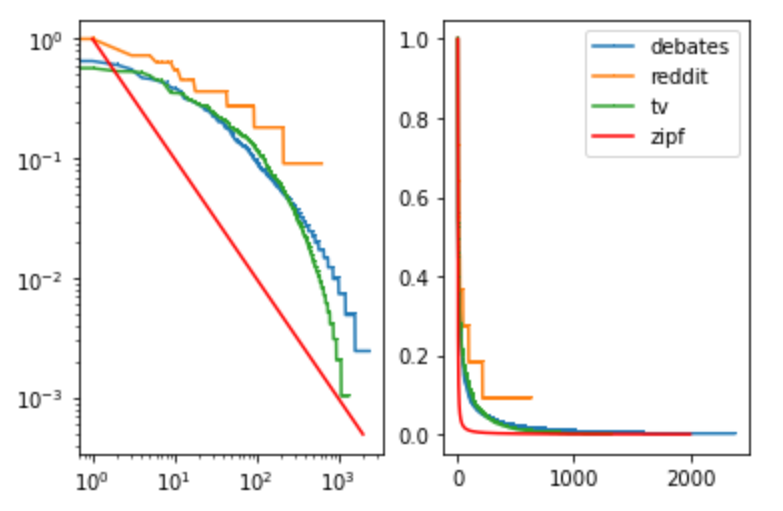
\includegraphics[width=0.8\linewidth]{zipf.png}
\end{figure}

\paragraph{\ild{Elements of language}} We can have different points of view on
language:
\begin{itemize}
\item Phonetics (sound)
\item Grammar
\begin{itemize}
\item Phonology
\item Morphology
\item Syntax
\end{itemize}
\item Semantics (meaning)
\end{itemize}

\paragraph{\ild{Morphology}} How words are built up from smaller meaningful
units, for instance \textit{un-lady-like}, \textit{dog-s}
\begin{itemize}
\item \textbf{\ild{Inflection}} -- variation in the form of a word (usually affix)
  that expresses a grammatical contrast
  \begin{itemize}
  \item adds tense, number, person, mood, aspect, etc
  \item e.g. \textit{run}$\rightarrow$ \textit{run} | \textit{running} 
  \item does not change word class
  \end{itemize}
\item \textbf{\ild{Derivation}} -- formation of a new word from another
  \begin{itemize}
  \item e.g. nominalization (\textit{computer}$\rightarrow$\textit{computerization})
  \item e.g. formation of adjectives (\textit{computational}, \textit{clueless})
  \item changes word class
  \end{itemize}
\end{itemize}

\paragraph{\textit{Morphemes}}
\begin{itemize}
\item \textbf{\ild{Root}} -- equivalence class of a word when all affixes are
  removed; not further decomposable into meaningful elements.
\item \textbf{\ild{Stem}} -- part of word that never changes when
  morphologically inflected, \iln{ i.e. without affixes describing tense, number,
  person, ... }
\item \textbf{\ild{Lemma}} -- Base form of word
\item From \textit{produced}, lemma is \textit{produce} but stem is \textit{produc}
\end{itemize}


\section{Tokenization}
 
\paragraph{\ild{Token}} an individual occurence of a word (as opposed to a
vocabulary/dictionary item)

\paragraph{\textit{Challenges}}
\begin{itemize}
\item Keep abbreviations, dates, numbers as single tokens
\item distuingish abbreviations from words
\item names and phrases (\textit{queen of england}, \textit{TU Wien})
\item compound words
\item apostrophes, umlauts, etc and other linguistic characteristics
\item encoding issues like RTL/LTR
\end{itemize}

\paragraph{\ila{Maximum Matching algorithm}} Use a dictionary of known terms.
Take the longest prefix of the input string that matches a dictionary item. Does
not always make sense (\textit{``Theta bled own there''}).

\section{Stemming}

\paragraph{\textit{Stemming/Lemmatization}} reduce tokens to equivalence
classes. Usually to gather words that are morphologically different but
semantically quite similar to the same set, i.e. to improve comparability. 

\paragraph{\ila{Porter Stemmer} } Rules for stripping suffixes. Applicability of
rules is based on \textit{measure} of a word $w$, which is the number $m$ s.t.
$w=C(VC)\{m\}V$ where $C,V$ are arbitrary sequences of consontants, vowels,
resp. --- Indeed reduces the words to their \textit{stems}.

\paragraph{\ila{WordNet \textsc{Morphy}} }
\begin{itemize}
\item Has  •  a sophisticated set of rules about inflections  • exception list
\item Checks the result of transformation against an extensive dictionary
\end{itemize}

\paragraph{\iln{Note}} \textsc{Morphy} reduces to \textit{lemmas}, while
\textsc{Porter} reduces to \textit{stems}.

\begin{itemize}
\item \textbf{\ild{Over-stemming}} Two words are reduced to the same root when
  they should not be
\item \textbf{\ild{Under-stemming}} Should be reduced to the same root but are not.
\end{itemize}


\section{POS-Tagging}

Given some input text and some tags (usually word types such as \textit{noun},
\textit{verb}, etc.), want to assign tags to tokens. (\textit{Sequence
  classification problem}).

Tagging can help with other procedures such as stemming, NER, parsing, ...

\paragraph{\ild{Def.}} Can divide words into two different classes
\begin{itemize}
  \item \textbf{\ild{Closed class}} --- can enumerate all members, e.g.
    determiners, pronouns, prepositions, ...
\item \textbf{\ild{Open class}} --- don't know all members, e.g. nouns, verbs,
  adjectives, ...
\end{itemize}

\paragraph{\iln{Note}}
\begin{itemize}
\item A single term (dictionary entry) can have different optimal POS-tags
  depending on its context.
\item Tagging helps to resolve ambiguities that exist on term-level (.e.g
  \textit{leaves} as \textsc{NN} or as \textsc{VB})
\item Tagging removes unnecessary distinctions e.g. all personal pronouns are
  \textsc{PRP}, determiners
\item Naive method (assigning most frequent tag in training data to term)
  already has 90\% accuracy.
\end{itemize}

\paragraph{\ild{Def.}}
\begin{itemize}
\item \textbf{\ild{Informativeness}} --- Assignment of tag adds information,
  reduces ambuigity
\item \textbf{\ild{Specifiability}} --- Ease of mapping a term to a tag
\item \iln{Example}: Collapsing multiple related tags into one decreases
  informativeness, decreases specifiability.
\end{itemize}

\paragraph{\textit{Feature selection}} Can look at word-local features (term,
pre-, suffixes, capitalization); but very often the tag of a word depends on its
context in the sentence.

\paragraph{\textbf{Main techniques}}
\begin{itemize}
\item \ild{Probabilistic tagging} --- consider lexical frequencies of tag in
  training data -- good when large training corpora are available
\item \ild{Rule-based tagging} --- use rules based on linguistic understanding
  -- good to tailor solution to very specific problems
\end{itemize}

\subsection{Probabilistic tagging}

Consider the definition of \ild{ conditional probability }
\begin{align*}
  P(A|B) = \frac{P(A,B)}{P(B)} 
\end{align*}
This gives rise to the \ild{chain rule}
\begin{align*}
  \Rightarrow P(A,B) = P(A|B) \cdot P(B)
\end{align*}
or, more generally
\begin{align*}
  P(w_1, ..., w_n) = \prod P(w_i~|~w_1, ..., w_{i-1})
\end{align*}
The problem here is that we cannot realistically obtain all the components of
the product because there are way too many possible sequences of words. Instead,
we employ the \ild{Markov assumption} that says that we can estimate the
probabilities by only consiering only the $k$ preceding terms
\begin{align*}
  P(w_i ~|~ w_1 ..., w_{i-1}) \approx P(w_i ~|~ w_{i-k}, ..., w_{i-1})
\end{align*}

For $k=1$, this yields the \ild{unigram model}, for $k=2$ the \ild{bigram model}
(i.e. $P(w_i | w_{i-1})$).

$n$-gram modelling is insufficient because language has \textit{long-distance depenencies}.

\paragraph{\ila{Unigram Tagger} } Assume that a unigram model generates the
current tagging. 

Assign a token $w$ its most frequent tag, i.e.
\begin{align*}
  t(w) := \argmax_t P(t~|~w)
\end{align*}
\textit{Improvement}: Use Bayes' formula, i.e. $P(A|B) = \frac{P(B|A)P(B)}{P(B)}$,
omitting the quotient:
\begin{align*}
  t(w) := P(t~|~w) = \argmax_t P(t) \cdot P(w~|~t)
\end{align*}

\paragraph{\textit{ \todo }} example

\paragraph{\ila{$n$-gram tagger} } Use information about the previous $n$
tokens in addition to information about current token. Can have \ild{word-based}
and \ild{tag-based} (tags are more common, training data covers more ground).

Assume a bigram language model (generating the sequence of POS-tags).

Pick the tag $t_i$ for word $w_i$ that maximises
\begin{align*}
  P(t_i ~|~ t_{i-1}) \cdot P(w_i~|~t_{i-1})
\end{align*}

For finding $P(t_i~|~t_{i-1})$, use the \ild{Maximum Likelihood Estimate} (where
$c$ is the count of observations)
\begin{align*}
  P(t_i | t_{i-1}) \approx \frac{c(w_{i-1}, w_i)}{c(w_{i-1})}
\end{align*}
\iln{(Use start and end symbols to be able to calculate probs for first and last
  words)}

% For $n=2$, can imagine a twodimensional lookup table:
% \begin{align*}
%   \text{previously seen POS-tag} \times \text{current word} \rightarrow 
% \end{align*}

\paragraph{\textit{\todo}} example


\subsection{Rule-based tagging}

Try to incorporate linguistic insight.

\paragraph{\ila{Brill tagger} }
\begin{enumerate}
\item Tag each word using a \ild{ baseline tagger } (e.g. unigram tagger, i.e.
  most common tag)
\item Apply patches that improve the result
  \begin{itemize}
  \item e.g. \textit{if one of the two preceding words is a determiner, change
      the tag from verb to noun}
  \item Based on training data, compute the error between any two
    should-be/is-assigned: $(t_a, t_b, \mathit{freq})$.
  \item For each error triple, apply the patch that results in the greatest
    improvement, apply it.
  \item Repeat until no further improvement is possible.
  \end{itemize}

\end{enumerate}



\section{Parsing}

\textit{We try to determine the grammatical structure of a sentence.}

\paragraph{\ild{Parsing problem}} Identify the parse tree (w.r.t some grammar)
for a given sentence. \iln{(There may be multiple parse trees, or none.)}

\paragraph{\ild{Parse tree}} depicts derivation of sentence beginning from start
symbol. Obviously requires context-free grammar \iln{(each set of children has
  exactly one parent)}

\paragraph{\textit{Motivation}}
\begin{itemize}
\item Grammar checking
\item Question answering
\item Machine translation
\item ...
\end{itemize}

\subsection{Constituency parsing}

\paragraph{\textit{Basic assumption}} Language is made up of \ild{constituents},
i.e. basic, nested building blocks \iln{(terminals and nonterminals of a formal grammar.)}

\paragraph{\ila{Leftmost derivation}} Always expand the leftmost expandable
nonterminal.

\paragraph{\ila{Shift-reduce parser}} \textit{(bottom-up approach)} Push tokens
onto stack until top of stack matches the \textit{rhs} of a rule, then reduce
(on stack). Accepts the word if start symbol alone is left on the stack.

\paragraph{\ild{Chomsky normal form}} The \textit{rhs} of a rule is of one of
these shapes
\begin{itemize}
\item $A \rightarrow BC$
\item $A \rightarrow a$
\item $S \rightarrow \varepsilon$
\end{itemize}


\paragraph{\ila{CYK Parser} } \textit{(dynamic programming, bottom-up)} Assumes
a grammar in CNF, i.e. \textit{rhs} of rules is two nonterminals or a terminal.
From the bottom up, in a dynamic programming fashion, remember if two subcells
are the \textit{rhs} of a production rule. The topmost cell produces the entire sentence.
\begin{figure}
  \centering
  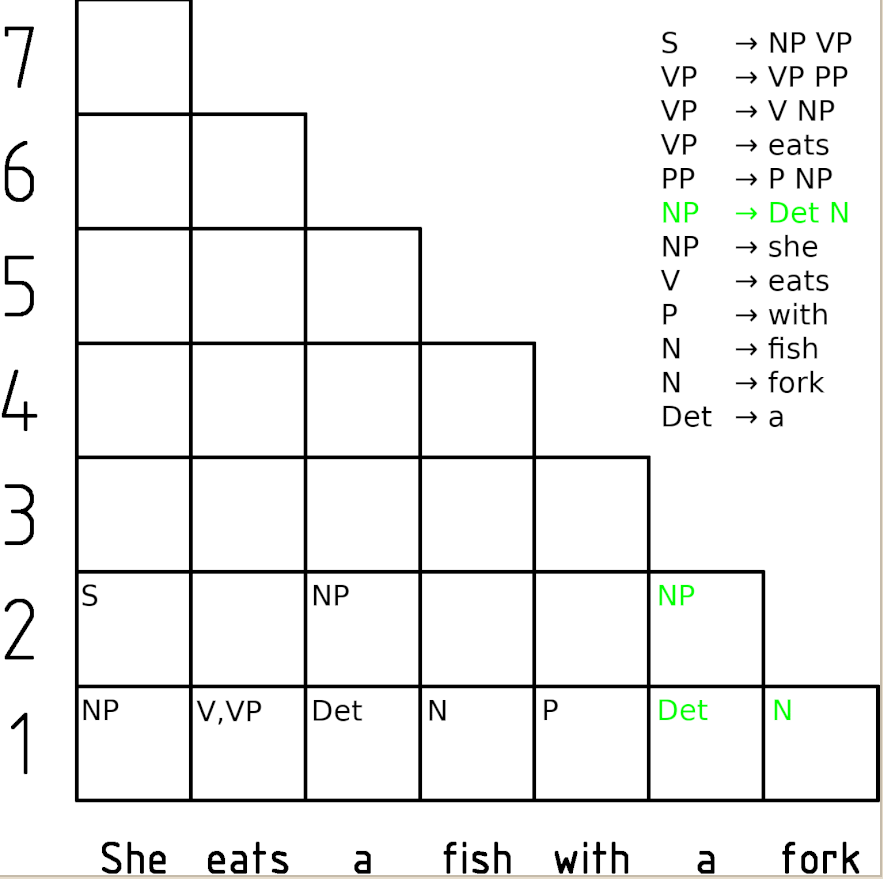
\includegraphics[width=0.4\linewidth]{cyk-parsing}
\end{figure}
Note that this finds all possible parse trees.

\subsection{Statistical Parsing}

\textit{Motivation: Sentences can have many different parse trees but some are
  clearly more likely than others.}

\paragraph{\textit{Basic idea}}
\begin{itemize}
\item Associate rules of a grammar with probabilities
\item The probability of a parse tree is the product of all used
  productions/derivations.
\item Probability of a sentence is the sum of all possible parse tree
  probablities.
\item Probabilities can be learned from a training corpus.
\item Can use probabilites in parsing algorithms such as the CYK parser to find
  the most likely parse tree.
\end{itemize}

\paragraph{\ild{Lexicalised Parsing}} Extend production rules to be specific to
terms (e.g. \textit{VP(ate)  $\rightarrow$ VP(ate) PP(with)}). Then, again,
assign/learn probabilities. \todo Head of sentence

\subsection{Dependency Parsing}

\paragraph{\textit{Basic concept}} Dependencies (in the linguistic sense)
between tokens (such as \textit{determiner, subject, ...}), these form a tree.
Again, want to find the most likely parse/dependency structure

\paragraph{\ila{Constraint-based Parsing} } Come up with rules describing what a
dependency can possibly look like. Begin with a complete graph of pairwise
dependencies, then iteratively eliminate dependencies according to rules.

\paragraph{\ila{Global linear models} } Assign a \ild{local feature vector}
$g(x,h,m)$ to a specific dependency $(h,m)$ in a specific sentence $x$. Try to
maximise the (weighted) sum of all depenencies in the sentence, i.e. the best
parse $y = F(x)$ is given by
\begin{align*}
  F(X) = \argmax_y \vec w \cdot \sum_{(h,m)\in y} g(x,h,m)
\end{align*}


\pagebreak
\part{Similarity Measures}

\textit{As there are many different expressions for the same semantic concept,
  we want to derive concepts of similarity between words. Further, this is
  useful in spelling correction.}

\section{Word similarity}

\paragraph{\ild{Phonological similarity}} How much do two words sound alike?

\paragraph{\ila{Soundex} } Reduce a given term/word into a phonetic
representation based on rules.

\paragraph{\ild{Morphological similarity}} basically comes down to stemming.

\paragraph{\ild{Spelling similarity}} Mainly want to identify spelling errors

\paragraph{\ila{Levenshtein distance / edit distance}} (\textit{dynamic
  programming}) We already know this. Extensions: Cost matrices, based for
example on distance of letters on keyboard.

\paragraph{\ild{Semantic similarity}} 
\begin{itemize}
\item \ild{Synonym} -- same meaning. A \ild{synset} is the equivalence class of synonymity.
\item \ild{Antonym} -- opposite meaning
\item \ild{hypernym} -- more general meaning
\item \ild{hyponym} -- more specific
\item \ild{meronym} -- part of collective
\end{itemize}

\paragraph{\ila{WordNet}} provides a tree (forest) of semantic relationships
between words. Similarity between $v,w$ can then be defined e.g. \todo


\section{Document similarity}

\paragraph{\ild{Vector space model}} See IR lecture notes.

\paragraph{\ild{tf-idf weight}} \begin{itemize}
\item \ild{term frequency $\mathit{tf}(t,d)$} --- How often does term $t$ appear in
  document $d$? Commonly dampened by logarithm.
\item \ild{document frequency $\mathit{df}(t)$} --- In how many documents does $t$ appear?
\item \ild{inverse document frequency $\mathit{idf}(t)$}  ---
  The basic idea: Rare terms are more informative
  than frequent terms and should thus receive a high score.  Thus we do the
  inverse fraction and log-dampening:
  \begin{align*}
    \mathit{idf}(t) := \log \frac{n}{\mathit{df}(t)}
  \end{align*}
\end{itemize}
The tf-idf weight is given by the product of term frequency and inverse document
frequency:
\begin{align*}
  \mathit{tf.idf}(t,d) = \log(1 + \mathit{tf}(td)) \cdot \log \left( \frac{n}{\mathit{df}(t)} \right)
\end{align*}
\begin{itemize}
\item term frequency increases with the number of occurences in the document
\item inverse document frequency increases with the rarity of the term in the collection
\end{itemize}

The score for a multi-term query and a document is
\begin{align*}
  \mathit{score}(q,d) := \sum_{t \in q \cap d} \mathit{tf.idf}(t,d)
\end{align*}
Problems:
\begin{itemize}
\item Bag-of-words model, does not consider order
\item Score is a sum, longer documents receive higher score
\end{itemize}

\paragraph{\ild{Vector space model}} Each document is a vector consisting of
tf-idf weights of terms. \ild{Distance measure}:
\begin{itemize}
\item euclidean distance is not suited because it considers the lengths (norms)
  of vectors, but we only really care about the distribution of terms
\item hence use \ild{cosine similarity}, which measures the angle between vectors.
\end{itemize}


\pagebreak
\part{Language Modelling}

\paragraph{\ild{Basic pipeline}}
\begin{enumerate}
\item Corpus
\item high-dimensional vector space
\item latent space (word embedings)
\item word relationships
\end{enumerate}


\paragraph{\ild{Word embedding}} Encode some notion of similarity to other words
in a vector. Motivation: Approaches like WordNet are static and thus
insufficient. Possible information
\begin{itemize}
\item syntactic similarity (\textit{run, ran})
\item semantic similarity (\textit{large, big})
\item relatedness (\textit{coffee, cup})
\end{itemize}

\paragraph{\ild{Word context matrix}} (\textit{co-occurence matrix})
\begin{itemize}
\item Each row represents a word
\item Each column represents some ``context'' (specific entity or other word)
\item cell represents the strengh of association, for example \textit{pointwise
    mutual information}
\end{itemize}
This matrix is very sparse. We'd like to find a low-dimensional
representation of our word vector (word embedding). We project into a
lower-dimensional space, the so-called \ild{latent space}.

\paragraph{\ila{Word2Vec}} \textit{(neural network for learning word vectors,
  context-independent model)}
Given a training corpus, every word in a fixed vocabulary is represented by a vector.
\begin{enumerate}
\item For each center word $c$ and a context window of fixed size $o$...
\item use the word vector similarity of $c$ and $o$ to calculate $P(o|c)$ (or
  $P(c|o)$, see below)
\item Adjust word vector to maximise predictive accuracy
\end{enumerate}
\begin{itemize}
\item \ild{Continous Bag-of-Words} (CBOW) learns $P(c|o)$, i.e. focus word given
  the context
\item \ild{Skip-gram} learns $P(o|c)$, i.e. context given some focus word.
\end{itemize}
Limitations:
\begin{itemize}
\item Any given word is represented by a vector which has to be stored
\item Polysemy (different meanings of same word) is not adressed at all
\item Dependence of meaning on context is not considered (gives rise to
  \ild{context-dependent models})
\end{itemize}

Given some word embeddings, how do we determine their similarity?
\begin{itemize}
\item similarity measures like cosine similarity
\item visualise by dimension-reduction techniques like t-SNE, PCA, MDS, UMAP,
  ...
\end{itemize}

\begin{itemize}
\item \ild{context-independent models} output a single word vector for a word
\item \ild{context-dependent models} generate multiple word embeddings for a
  word that capture different contexts.
\end{itemize}

\paragraph{\ild{Sentence embedding}} \begin{itemize}
\item Basic approach with Bag-of-words assumption, vector of tf-idf weights -- Problems:
  \begin{itemize}
  \item problem: vectors are large and very sparse
  \item cosine similarity of sentences with distinct words is zero but there
    could still be semantic similarity.
  \end{itemize}
\item Average word embeddings
\item Deep learning approaches
\end{itemize}

\paragraph{\textit{Applications}}
\begin{itemize}
\item Assistants like Google, Siri, Alexa, ... for understanding an generating
  language, answering questions, ...
\item Opinion mining
\item Sentiment analysis
\item Named Entity Recognition
\end{itemize}

\paragraph{\textit{Limitations}} Language models potentially contain biases
(ethnic, gender) induced by the training data.






\pagebreak
\part{Text Data Mining}

\pagebreak
\part{Opinion Mining \& Information Extraction}

\section{Information Extraction}

to extract  • the entities and  • relationships between such entities (i.e.
clear, factual information)

\subsection{Named Entity Extraction}

used for  • summarizing text  • answering questions  • integrating into knowlege
bases  • associating information (e.g. sentiments) to sentiments (e.g. of parts
of printer in question)

Possible types of entities  • location  • time  • person  • ...

\paragraph{\textit{Supervised learning models}} Based on labelled training
sequences (of tokens), train a classifier to predict labels (\textit{Sequence
  Labelling Problem})
\begin{itemize}
\item new data must fit training data
\item time-consuming
\end{itemize}

To make this easier, use features that go beyond single tokens, e.g. context
window of $k$ words.

\paragraph{\textit{Sequence Labelling}}  • reminiscent to POS-tagging  • assuming
that label is dependent on context. Typical models are  • Markov models  •
Conditional Random Fields  • Bidirectional LSTMs

Once we have identified the entities, we'd like to find relationships between
them (e.g. triples of operators \textit{is-a}, \textit{daughter-of}, ...)
\iln{(Can save these triples in a knowledge base e.g. for question-answering; cf
  \textsc{Rdf}-triples)}.

\paragraph{\textit{Relationship Extraction}} Try to find type of relationship
between two entities. Possibilities
\begin{itemize}
\item Extract \textsc{Rdf} triples from large corpora like Wikipedia
\item Use (specialised) ontologies / knowledge bases (for ex. medical applications)
\end{itemize}
Methods to extract information:
\begin{itemize}
\item handwritten rules -- e.g. \textit{``Y such as X'', ``X, especially Y'',
    ``X, including Y'' all express an \textit{is-a}-relationship}. -- there can
  be more specific relations that only make sense between certain types of
  entities (e.g. \textit{cures(drug, disease)}) -- pros:  • precise  • can be
  tailored to specific domains -- cons:  • low recall  • high effort
\item supervised,
\item unsupervised machine learning.
\end{itemize}

semi-supervised learning: extract less common patterns based on training corpus?






\pagebreak
\part{Question Answering \& Text Summarization}


\end{document}